\documentclass{article}


\usepackage{arxiv}

\usepackage[utf8]{inputenc} % allow utf-8 input
\usepackage[T1]{fontenc}    % use 8-bit T1 fonts
\usepackage{hyperref}       % hyperlinks
\usepackage{url}            % simple URL typesetting
\usepackage{booktabs}       % professional-quality tables
\usepackage{amsfonts}       % blackboard math symbols
\usepackage{nicefrac}       % compact symbols for 1/2, etc.
\usepackage{microtype}      % microtypography

\usepackage{graphicx}	% to insert graphs
\usepackage{caption}	% to customize caption style
\usepackage{float}
\usepackage{subfigure}


\title{Predicting the Outcome of 2020 English Premier League (EPL) Football Matches}


\author{
 Group Name: \texttt{Group D}\\
  Department of Computer Science\\
  University College London\\
  London, WC1E 6BT\\
}


\begin{document}

\maketitle
\captionsetup[figure]{labelformat={default},labelsep=period,name={Fig.}}


% -------------------------------------------------------------------------------------------
\section{Introduction [Terry] }


% -------------------------------------------------------------------------------------------
\section{Data Transformation \& Exploration [Yun]}

At first sight, we found that:
\begin{itemize}
\item The shape of the data frame is 4180 rows x 73 columns, but some columns are empty and unnamed.
\item There are two different date formats, "\%d\/\%m\/\%y" and "\%d\/\%m\/\%Y".
\item The involved data is from 2008-08-16 to 2019-05-12 (i.e. totally 11 seasons).
\end{itemize}

\begin{figure}[ht]
\centering
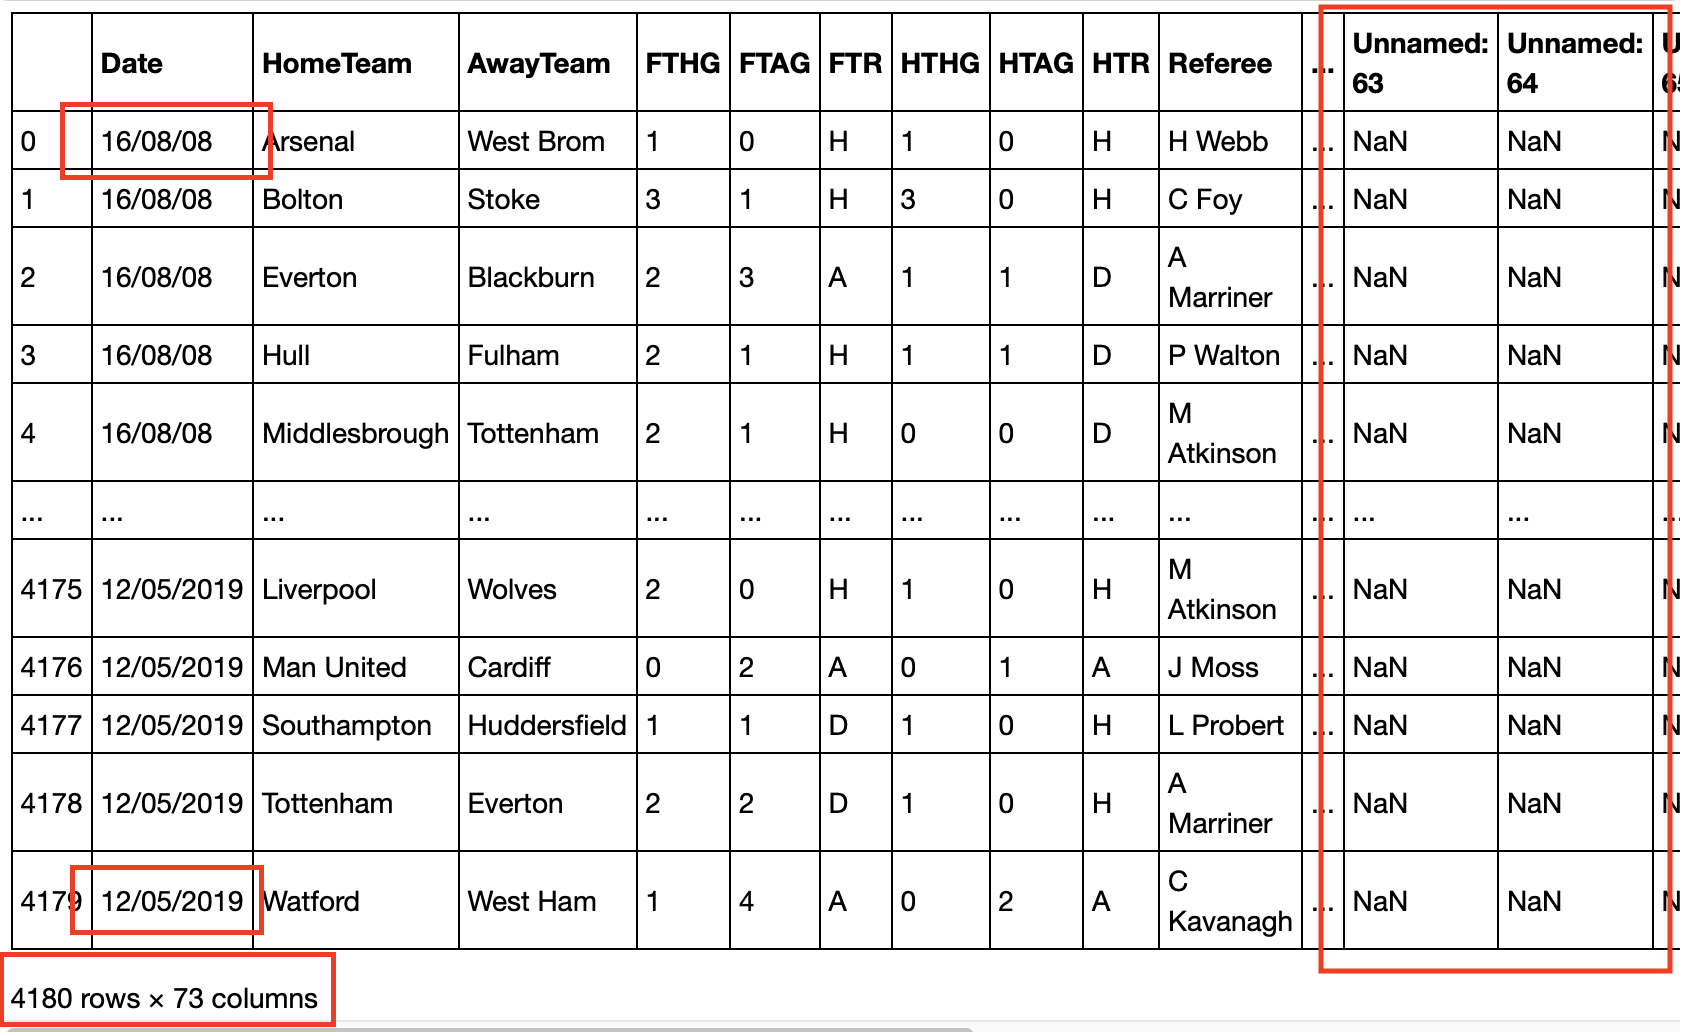
\includegraphics[scale=0.4]{graphs/firstSight.png}
\caption{ First sight of training data}
\label{fig:firstSight}
\end{figure}

% -------------------------------------------------------
\subsection{Data Cleaning}

After we dropped the unnamed columns, the number reduced to 22.

We verified that there is no row containing invalid values (i.e., None, NaN, infinite or overflowed number), so we don’t need to drop any rows. The size remains 4180.

We then unified the date formats, converting into “\%Y-\%m-\%d” for later exploration and transformation.
% -------------------------------------------------------
\subsection{Initial Data Exploration}
% ----------------------------
\subsubsection{Number of matches per season}
The full set is of huge amount. To help learn the data, we separated rows by date from August to May (i.e., one season) to check how many matches there are per season.
\begin{figure}[ht]
\centering
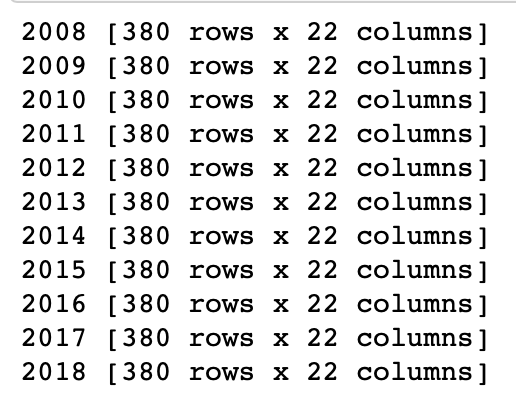
\includegraphics[scale=0.6]{graphs/matchesPerSeason.png}
\caption{Number of matches per season}
\label{fig:matchesPerSeason}
\end{figure}

We found that the number of matches each season stays constant (380).

% ----------------------------
\subsubsection{Percentage of match result}

We also computed the average percentage of each match result per season and that over the 11 years. See Fig. \ref{fig:FTRPercentage}

\begin{figure}[H]
\centering  
\subfigure[]{
\label{Fig.sub.1}
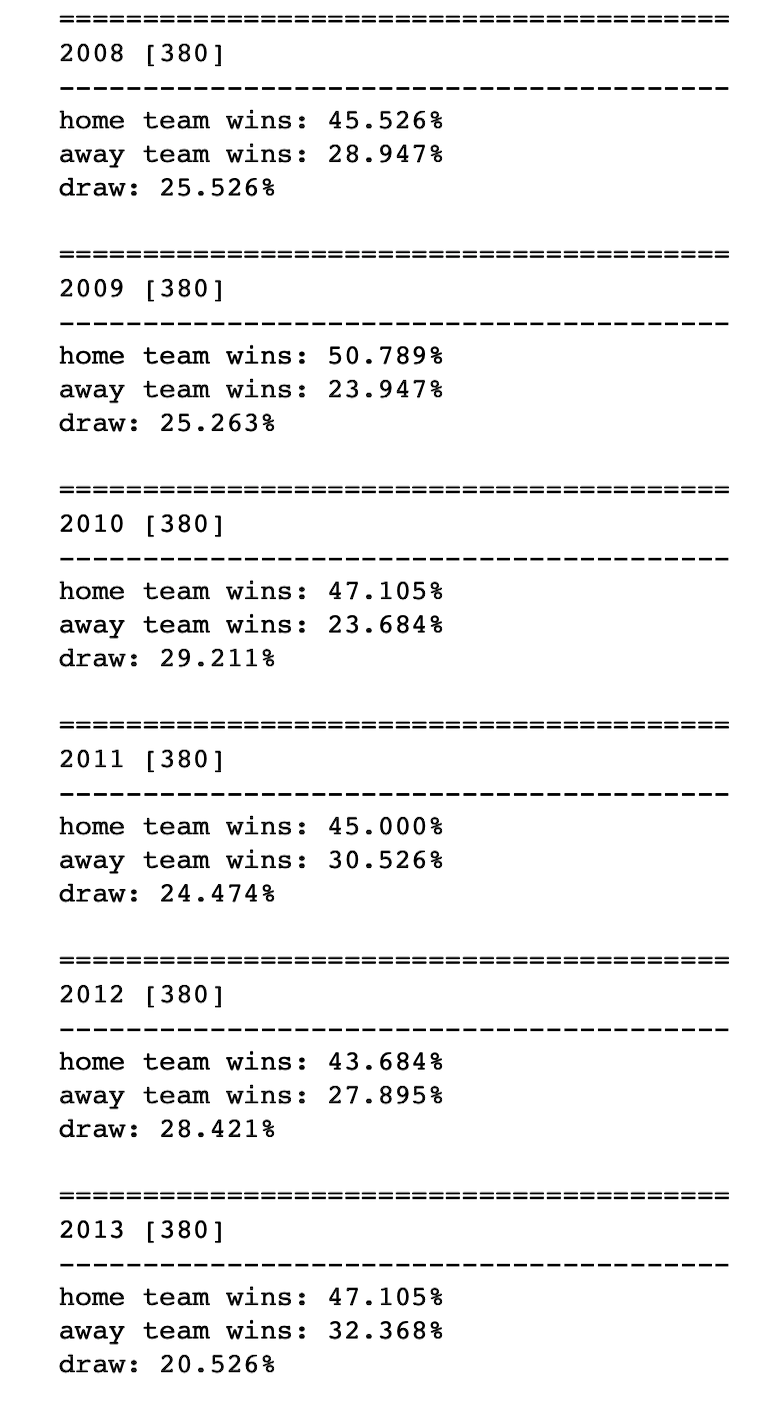
\includegraphics[width=0.45\textwidth]{graphs/FTRPercentage1.png}}
\subfigure[]{
\label{Fig.sub.2}
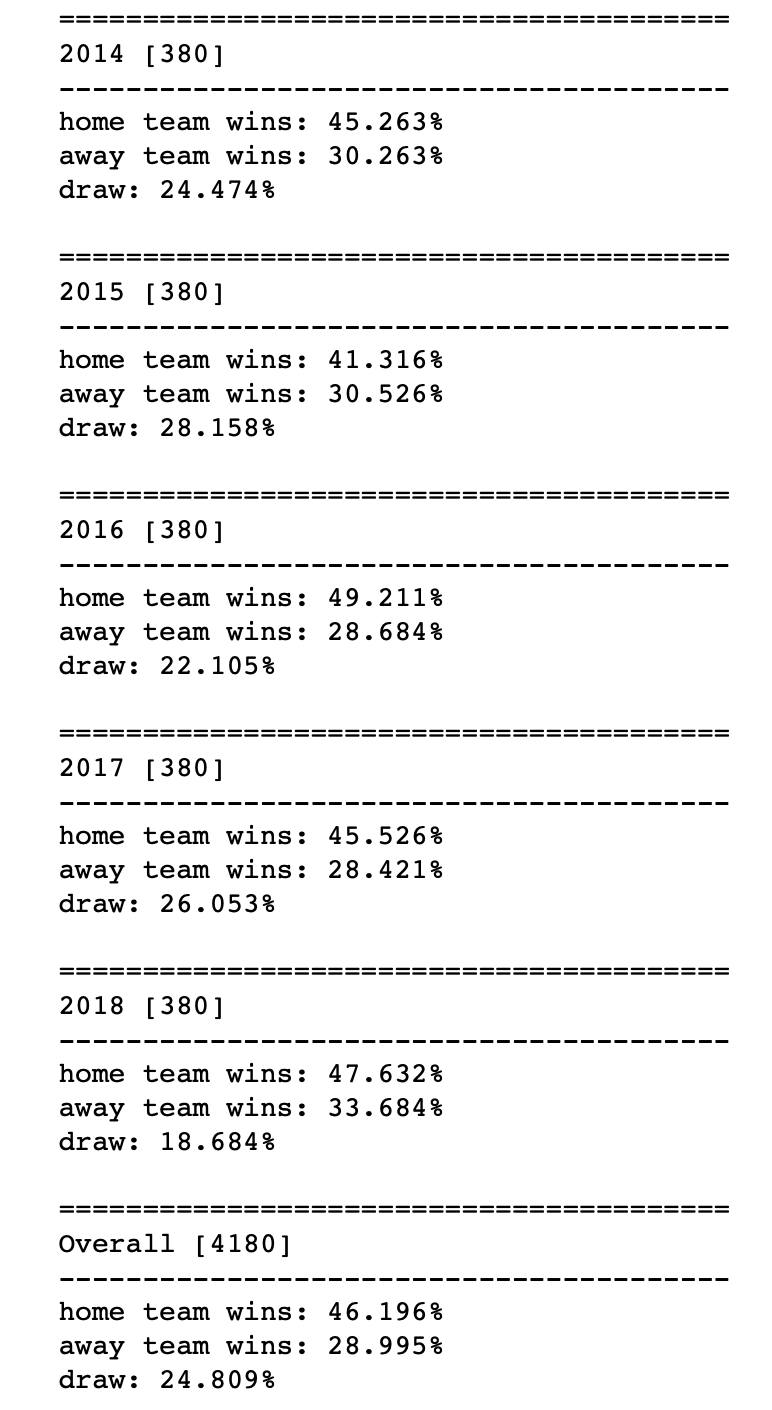
\includegraphics[width=0.45\textwidth]{graphs/FTRPercentage2.png}}
\caption{Percentage of each match result}
\label{fig:FTRPercentage}
\end{figure}

From the result we noticed that in all cases the result 'home team wins' (‘H’) is of the highest probability, and 'H':'A':'D' $\approx$ 5:3:2 in general.

% ----------------------------
\subsubsection{Relationship between attributes}
We plotted a Pearson Correlation Heatmap (Fig. \ref{fig:top-10-features-in-raw-data}) to see the top 10 features related to the match result (FTR).

\begin{figure}[ht]
\centering
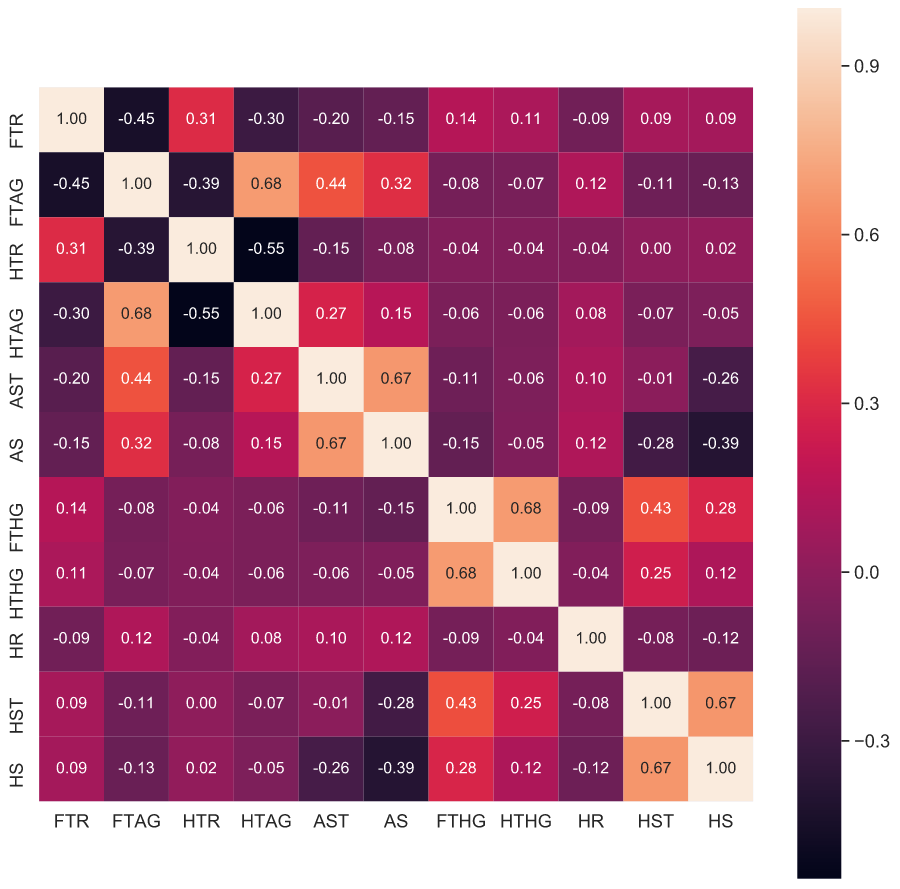
\includegraphics[scale=0.3]{graphs/top-10-features-in-raw-data.png}
\caption{The top 10 features related to FTR}
\label{fig:top-10-features-in-raw-data}
\end{figure}

As shown in the graph, the top 10 features are: \\
\centerline{HTR,  FTHG, HTHG, HST, HS, HR, AS, AST, HTAG, FTAG,}	\\
ordered from the greatest to least.

It is notable that the goal scored at full time (FTHG, FTAG)  \& goal scored at half time (HTHG, HTAG) and
the total number of shots on goal (HS, AS)  \& that on target (HST, AST) are the two pairs of data which are highly correlated (> 0.65).

% -------------------------------------------------------
\subsection{Feature Construction}
So, within the top 10 we picked FTHG, FTAG , HS, AS,  HR, AR to create features:
\begin{itemize}
\item FTHG, FTAG $\Rightarrow$ the cumulative full-time goal difference by home team and away team [HCGD, ACGD]
\item HS, AS $\Rightarrow$  the average number of shots on goal in the past 3 matches by home team and away team [HAHS, AAHS]
\item HR, AR (as features directly) 
\end{itemize}

Apart from that, we also derived features from the following attributes:
\begin{itemize}
\item Date $\Rightarrow$  the delta time from last match of home team and away team  [HDT, ADT]
\item HomeTeam, AwayTeam $\Rightarrow$  the distance needed to travel for the away team (with the help of extra data source) [DIS]
\item FTR $\Rightarrow$ the performance of past 3 matches of the home team and away team [HM1,AM1, HM2,AM2. HM3,AM3]
\end{itemize}

Due to the lack of data in the beginning of each year, there are a few rows containing empty values. After removing these rows and also the intermediate data (which we used to create features), the feature set is shown in  Fig. \ref{fig:featureSet}.

\begin{figure}[ht]
\centering
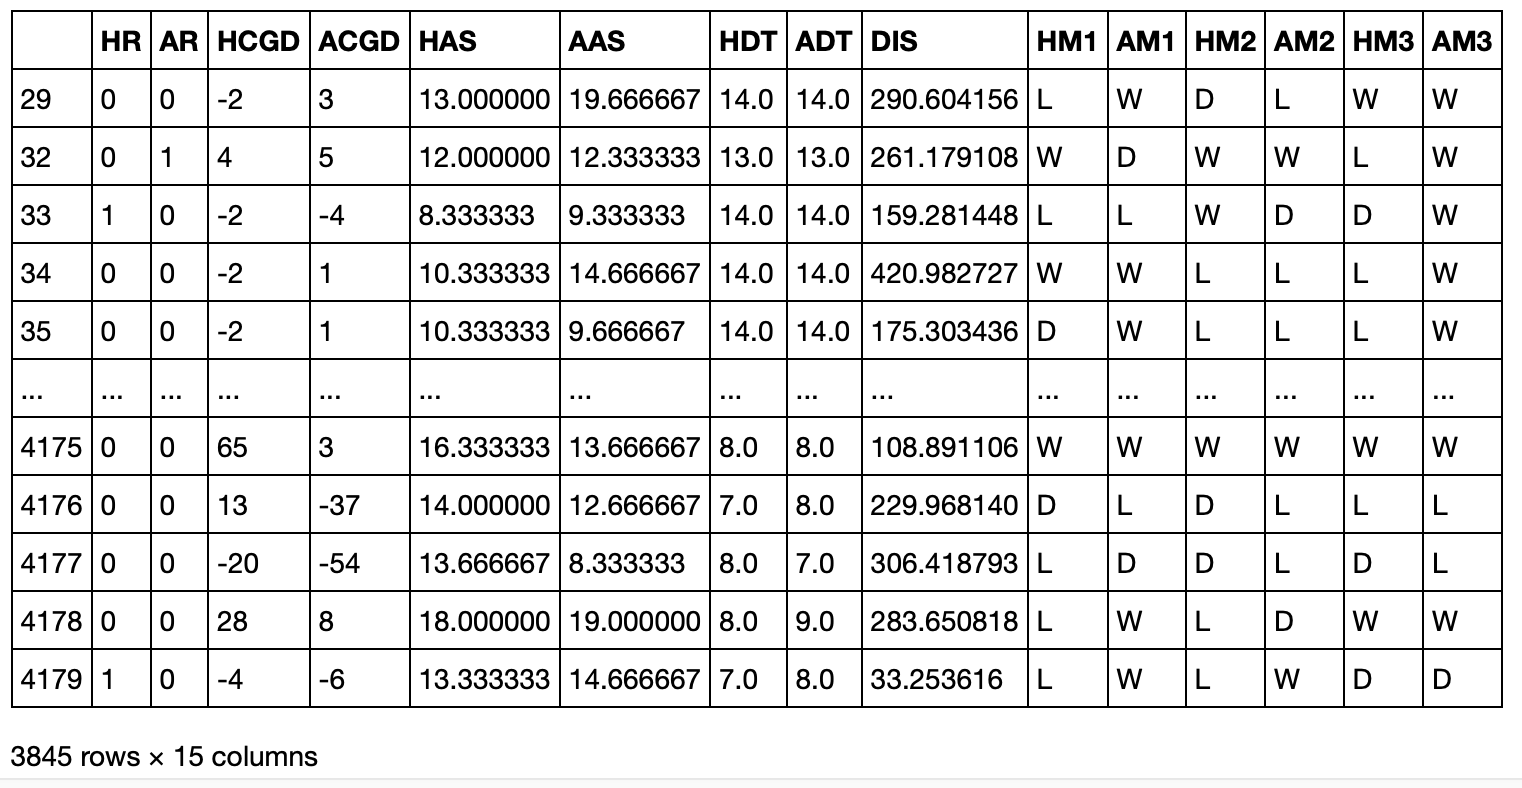
\includegraphics[scale=0.5]{graphs/featureSet.png}
\caption{Feature set}
\label{fig:featureSet}
\end{figure}

% -------------------------------------------------------
\subsection{Second Data Exploration - Analyse Numerical Features}
To learn the characteristics of each feature, we derived the minimum, maximum, median, mean, variance and standard deviation:
\begin{figure}[H]
\centering  
\subfigure[]{
\label{Fig.sub.3}
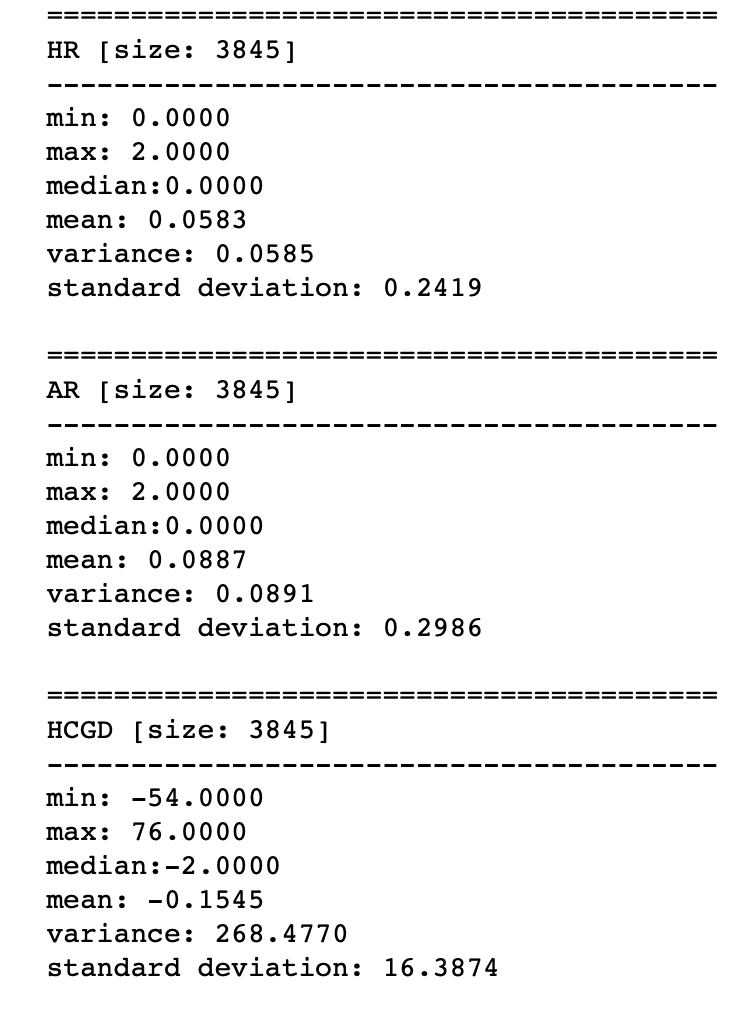
\includegraphics[width=0.32\textwidth]{graphs/statistics1.png}}
\subfigure[]{
\label{Fig.sub.4}
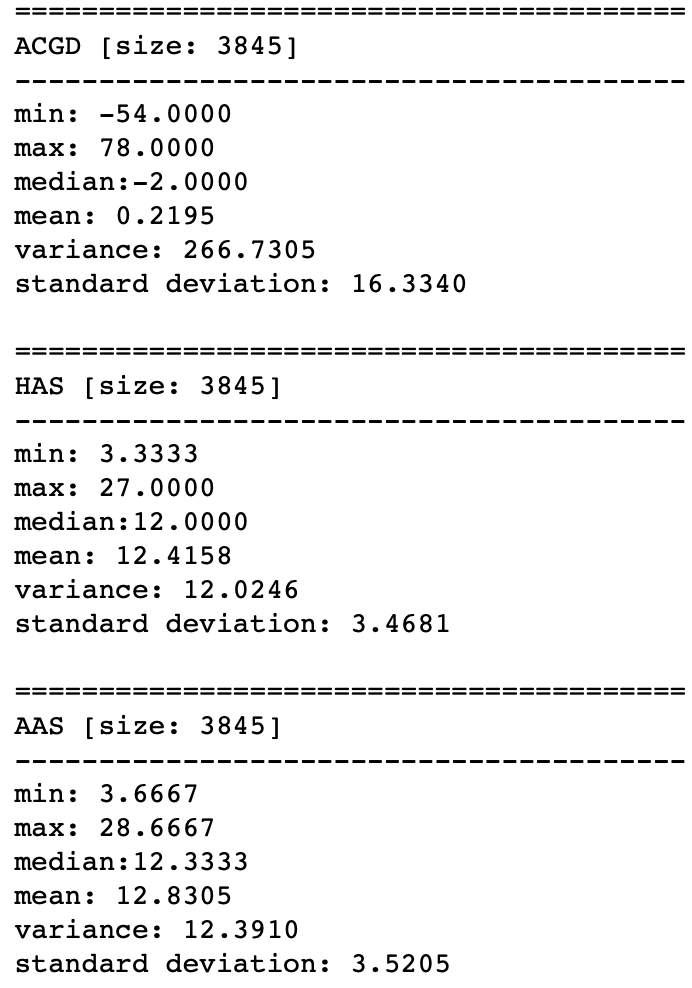
\includegraphics[width=0.32\textwidth]{graphs/statistics2.png}}
\subfigure[]{
\label{Fig.sub.5}
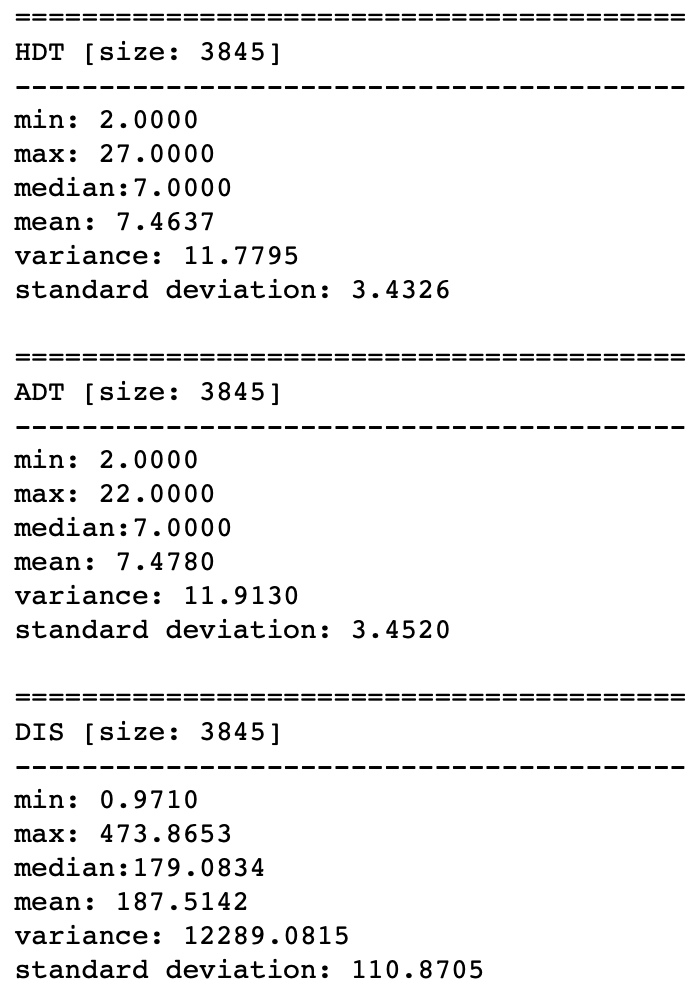
\includegraphics[width=0.32\textwidth]{graphs/statistics3.png}}
\caption{ Statistics of each feature column}
\label{fig:statistics}
\end{figure}

From the figure, we can draw such conclusions:
\begin{itemize}
\item HR \& AR: The range is very small (2). From the median, the mean and also the small variance we can know that most values are 0 (as these two features are discrete) while value=2 is of low occurrence.
\item HCGD \& ACGD: Large range (> 130) with negative values involved. The median and the mean demonstrates that there is a relatively greater number of negative values within the data set.
\item HAHS \& AAHS: Moderate range (around 25) with all positive values. The median and the mean is at the half of the range while the variance is reasonable.
\item HDT \& ADT: Similar moderate range (around 25) and variance with the above pair of data. But the median and the mean is at the one third of the range. Outliers may exist.
\item DIS: Large range (> 450) with all positive values. Reasonable median and mean. But from the variance we can know that the value fluctuates significantly.
\item Comparing to the other features, the values of HR \& AR are too small while that of DIS too large.
\end{itemize}

% -------------------------------------------------------
\subsection{Data Transformation}
% --------------------------------------
\subsubsection{Label mapping}
We mapped the label (i.e., FTR) into numbers for later model training by the rule:
\begin{itemize}
\item 'H' $\to$ 1
\item 'A $\to$ 0
\item 'D' $\to$ 2
\end{itemize}

% ------------------------------------
\subsubsection{Rescale and standardize numerical features} \label{`}
With the conclusions from 3.3, we applied the z-score standardization and min-max rescaling to the numerical features.
% -----------------------------------
\subsubsection{Transform categorical features}
The categorical data within the feature set is: \\
		\centerline{HM1,AM1, HM2,AM2, HM3,AM3, }\\
which only take the values {‘W’, ‘L’, ‘D’}.

So we introduced the binary features		\\
\centerline{HM1\_W, HM1\_L, HM1\_D}	\\
\centerline{AM1\_W, AM1\_L, AM1\_D}		\\	
\centerline{......}		\\
\centerline{AM3\_W, AM3\_L, AM3\_D}		\\
such that if, for example, HM1 takes the value of ‘W’,  then HM1\_W = 1, HM1\_L= 0, HM1\_D = 0. 

% -------------------------------------------------------------------------------------------
\section{Methodology Overview [Yanke]}



% -------------------------------------------------------------------------------------------
\section{Model Training \& Validation [Yanke]}



% -------------------------------------------------------------------------------------------
\section{Results [Yi]}



% -------------------------------------------------------------------------------------------
\section{Final Predictions on Test Set [Yusi]}


% -------------------------------------------------------
\subsection{Data Pre-processing}

Before predicting the result we first need to process the test set to fit our model. We applied similar operations as we dealing with the training data. To derive features, we import the up-to-date data of the season 2019 from {\em<http://www.football-data.co.uk>} .

% -------------------------------------------------------
\subsubsection{Data cleaning}

For the up-to-date data, we first remove all the columns that are not presented in the training set, and then check if any invalid data involved.  As a result, the shape of the data set reduce from 209 rows x 106 columns to 209 rows x 22 columns.

The shape of test set is 10 rows x 3 columns. So we can get the result by simply looking at the data:
\begin{itemize}
\item It only contains three attributes which are all presented in the training set;
\item There is no rows containing None, NaN, inifinite or overflowed values.
\end{itemize}

We then concatenate the up-to-date data of season 2019 and the test set and unify the date. See Fig.\ref{fig:rawData2019}
\begin{figure}[ht]
\centering
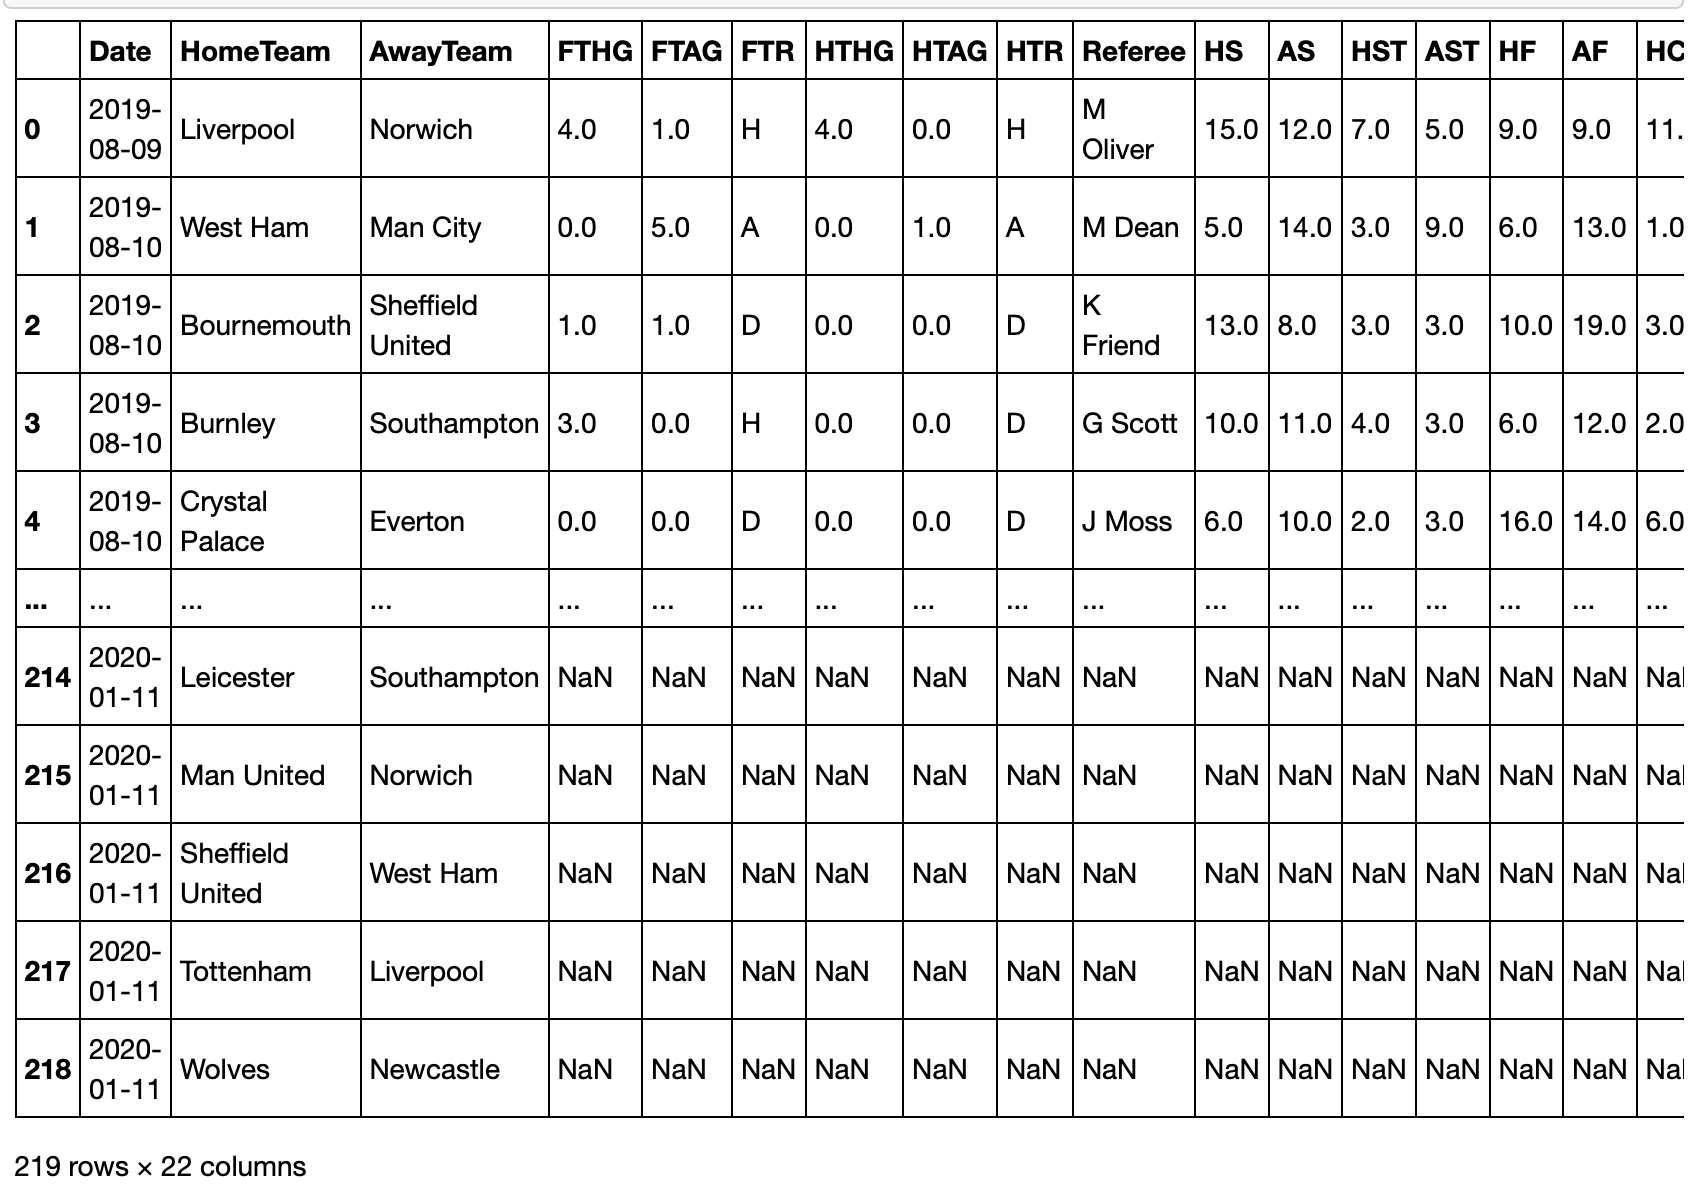
\includegraphics[scale=0.5]{graphs/rawData2019.png}
\caption{Data 2019}
\label{fig:rawData2019}
\end{figure}

% -------------------------------------------------------
\subsubsection{Feature derivation}
Same process with when we handle the training data: select the basic attributes, construct features, remove invalid data and remove intermediate data (i.e., the basic attributes).

% -------------------------------------------------------
\subsubsection{Data transformation}

We re-scale and standardise numerical features by using the scalers that are fitted with the training data in the previous step. Categorical features are transformed using the same rule as we transforming the training data.

% -------------------------------------------------------
\subsection{Result Prediction}
We can now make prediction using the final model we choose to use and the processed 2019 data set. The result is shown in the Fig.\ref{fig:encodedResult},
\begin{figure}[ht]
\centering
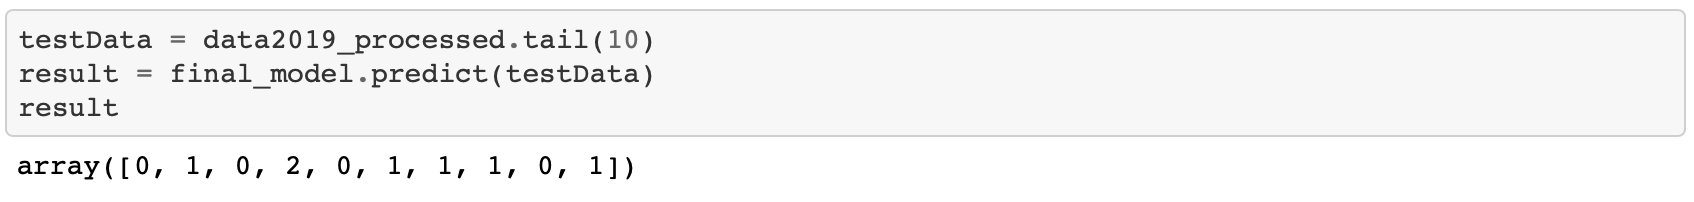
\includegraphics[scale=0.5]{graphs/encodedResult.png}
\caption{}
\label{fig:encodedResult}
\end{figure}

Where 1 means 'Home Team Wins', 0 means 'Away Team Wins', 2 means 'Draw'.

So our prediction is such that (Fig.\ref{fig:finalPrediction}):

\begin{figure}[ht]
\centering
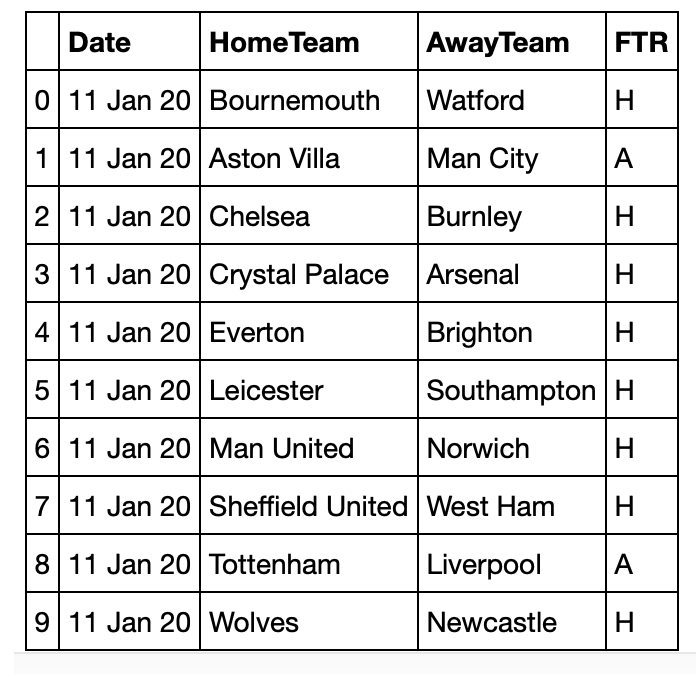
\includegraphics[scale=0.5]{graphs/finalPrediction.png}
\caption{}
\label{fig:finalPrediction}
\end{figure}

% -------------------------------------------------------------------------------------------
\section{Conclusion [Terry]}




% -------------------------------------------------------------------------------------------
\bibliographystyle{unsrt}  
%\bibliography{references}  %%% Remove comment to use the external .bib file (using bibtex).
%%% and comment out the ``thebibliography'' section.


%%% Comment out this section when you \bibliography{references} is enabled.
\begin{thebibliography}{1}

\bibitem{1}
Sharma, Mohit.
\newblock What Steps should one take while doing Data Preprocessing?.
\newblock June 20th 2018.
\newblock June 1st 2019.
\newblock {\em<https://hackernoon.com/what-steps-should-one-take-while-doing-data-preprocessing-502c993e1caa>}.

\bibitem{2}
J. González.
\newblock Scaling/ normalisation/ standardisation: a pervasive question.
\newblock Oct 18th 2018.
\newblock June 3st 2019.
\newblock {\em<https://quantdare.com/scaling-normalisation-standardisation-a-pervasive-question/>}.
  

\end{thebibliography}


% -----------------------------------------------------------------------------------------
\end{document}